%
% Tutorial -- BJT Modeling and Verification
%
% Copyright (C) 2005 Thierry Scordilis <thierry.scordilis@free.fr>
%
% Permission is granted to copy, distribute and/or modify this document
% under the terms of the GNU Free Documentation License, Version 1.1
% or any later version published by the Free Software Foundation.
%

\section*{warning}

\textit{
This chapter will describe an RF design issue using QUCS. The author assume that the basic manipulation of qucs is known. You will find herein mainly a MacOsX description that is close to a linux or unices architecture.
}


%-------------------------------------------------------------------------
\tutsection{choice of transistor}

The choice has been made to choose among the Philips RF wideband transistor library. These components are easy to find, with resonnable prices.

This list could be found at \texttt{http://www.semiconductors.philips.com/}.

A resume of these transistors can be found in the figure \ref{design:pa:toTable}
\begin{figure}[htbp]
\begin{center}
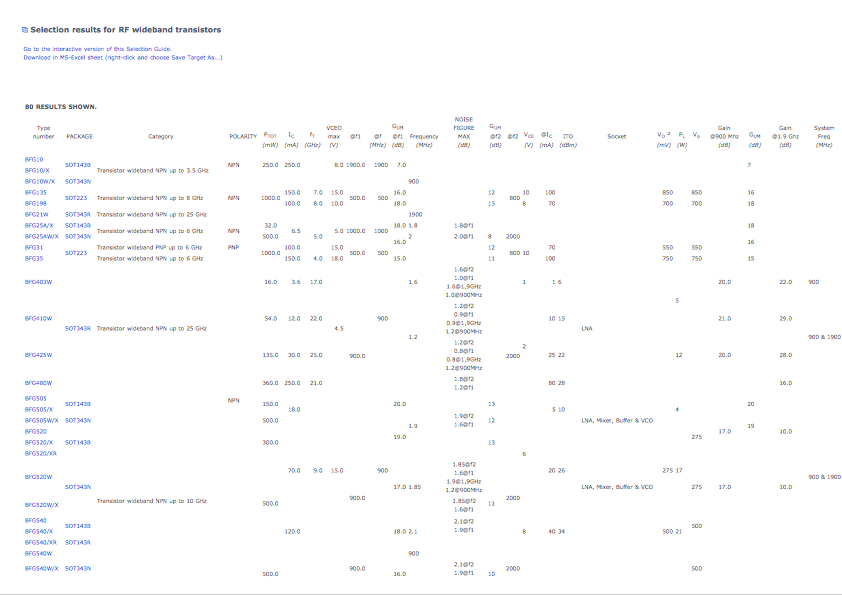
\includegraphics[angle=90,scale=0.7]{philipsTable}
\caption{transistor table from philips semiconductor}
\label{design:pa:toTable}
\end{center}
\end{figure}

I will not discuss herein, the reason \footnote{regarding current, $F_t$ , $V_{ce}$ , power dissipation, etc \ldots} why of the final choice, but the $BFG425w$ is the candidate. It offers high gain, with low figure noise ( if LNA consideration )  high transistion frequency ( 25 GHz ), its emitter is thermal lead, low feedback capacitance. This device could be used in RF front end, analog or digital cellular, radar detectors, pagers, SATV, oscillators. It is in a SOT343R package suitable for small integration.

The maximum acheivable gain is 20 dB with 25 mA, $V_{ce} = 2$ V at 2 GHz and $25^\circ C$. The third order intercept point in these conditions is typically $22 dBm$.

These parameter should be compatible with our need. Here are the spice parameter of the device.

\bigskip


\begin{verbatim}
.SUBCKT BFG425W 1 2 3 
L1   2 5 1.1E-09
L2   1 4 1.1E-09
L3   3 6 0.25E-09
Ccb  4 5 2.0E-15
Cbe  5 6 80.0E-15
Cce  4 6 80.0E-15
Cbpb 5 7 1.45E-13 
Cbpc 4 8 1.45E-13 
Rsb1 6 7 25 
Rsb2 6 8 19 
Q1 4 5 6 6 NPN 

.MODEL NPN NPN 
+ IS = 4.717E-17 	+ BF = 145    + NF = 0.9934 
+ VAF = 31.12 		+ IKF = 0.304 + ISE = 3.002E-13 
+ NE = 3 			+ BR = 11.37 	+ NR = 0.985 
+ VAR = 1.874 		+ IKR = 0.121 	+ ISC = 4.848E-16 
+ NC = 1.546 		+ RB = 14.41	+ IRB = 0 
+ RBM = 6.175 		+ RE = 0.1779 	+ RC = 1.780
+ CJE = 3.109E-13 	+ VJE = 0.9 	+ MJE = 0.3456 
+ CJC = 1.377E-13 + VJC = 0.5569 + MJC = 0.2079 
+ CJS = 6.675E-13 + VJS = 0.4183 + MJS = 0.2391 
+ XCJC = 0.5 		+ TR = 0.0 	+ TF = 4.122E-12 
+ XTF = 68.2 		+ VTF = 2.004 	+ ITF = 1.525 
+ PTF = 0 			+ FC = 0.5501 	+ EG = 1.11 
+ XTI = 3 			+ XTB = 1.5 
.ENDS

\end{verbatim}

Since the model used in SPICE and in QUCS rely on a gummel-poon modelisation, and since the level of modelisation is the same, some quite direct conversion could be used to create the library for QUCS.

To use directly this file, you will need to store the file in an other directory from the project one ( a small bug taken into account ). Then it should work but some there are still some issues on the parameters itselves, This is the reason why we will proceed in an other way.

The data sheet could be found on the philips web site. 

\begin{figure}[htbp]
\begin{center}
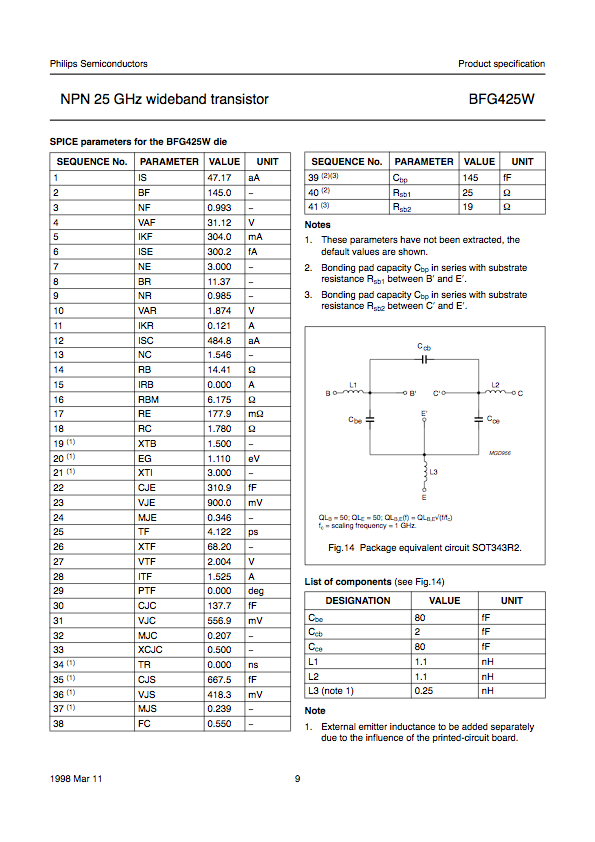
\includegraphics[scale=0.7]{spice_bfg425}
\caption{spice parameter extract from philips data sheet}
\label{design:pa:spiceDatasheet}
\end{center}
\end{figure}

%-------------------------------------------------------------------------

\tutsection{library creation}

Remember that when creating a device, it is almost always mandatory to read of have a look at on how the model is done is the technical documentation. It is very to understand the limitation, and how we can correct some data if needed. The mian pity is that a lot of commercial software are quite obscure on the real model they use and their limitation ; QUCS is quite exceptionnal  on this point this the complete modeling is explain theoretically in a special technical paper.

\bigskip

In order to conduct these test, we need to create a model of our component. To perform this you should create the file that contain all the libraries, this file is stored under 

\begin{verbatim}
/usr/local/share/qucs/library/philips_RF_widebande_npn.lib
\end{verbatim}

You can edit this file with \texttt{vi}. You need to add the following line :
\begin{verbatim}
<Qucs Library 0.0.7 "philips RF wideBand">

<Component BFG425W>
  <Description>
    RF wideband NPN 25GHz 
    2V, 25mA, 20dB , 2000MHz
    Manufacturer: Philips Inc.
    NPN complement: BFG425W
    --------------------------
    based on spice parameter from philips
    --------------------------
    sept 2005  thierry
  </Description>
  <Model>
<_BJT T_BFG425W_ 1 480 280 8 -26 0 0 "npn" 1 "47.17e-10" 
1 "1" 1 "1" 1 "0.304" 1 "0.121" 1 "31.12" 1 "1.874" 0 
"300.2e-15" 1 "3" 1 "484.8e-10" 1 "1.546" 1 "145" 1 "11.37"
1 "6.175" 1 "0" 1 "1.78" 1 "0177.9e-3" 1 "014.41" 1 "310.9e-15"
1 "0.900" 1 "0.346" 1 "137.7e-15" 1 "0.5569" 1 "0.207" 1 "0.500"
1 "667.5e-15" 1 "0.4183" 1 "0.239" 1 "0.550" 1 "4.122e-12" 1
"68.2" 1 "2.004" 1 "1.525" 1 "0.0" 1 "26.85" 1 "0.0" 0 "1.0" 0 
"1.0" 0 "0.0" 0 "1.0" 0 "1.0" 0 "0.0" 0>
  </Model>
</Component>
\end{verbatim}

You can replace the $1$ by $0$, this will remove the visible checkbox, the fact to place a $1$ first enable the user to change and or view the parameters that are being used.

A trick to provide all the required syntax is to fill a NPN into the schematics, perform a copy on the device, you should then have the model in the clipboard, just paste into to file and add the description and the markup language boundaries. The syntaxe is explained in the help at the topic \textit{description of the qucs file formats}.


Then the device is visible in the \texttt{Component Library Tool} as mentionned in figure \ref{design:pa:componentTool}.

\begin{figure}[htbp]
\begin{center}
	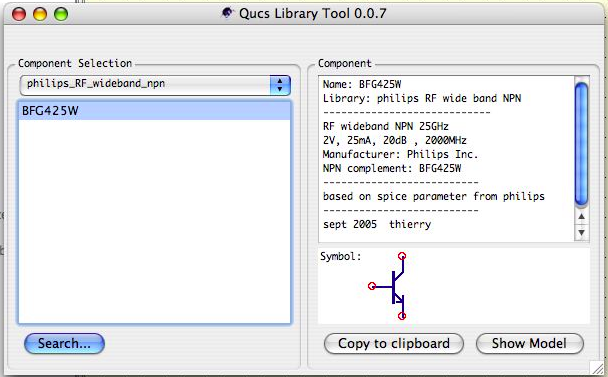
\includegraphics[scale=0.5]{componentLibrary}
	\caption{QUCS Component Library showing the new component}
	\label{design:pa:componentTool}
\end{center}
\end{figure}


By doing this you haved the possibility to reuse the device as much as you want, and you can debug devices in a more easy way.

\underline{\textbf{Warning}} : in this section we have only describe the die of the device, for the parasitic from the package, we will be obliged to describe this circuit, but later on.

\tutsection{device library verification}

The first step, before using the device in a application, is to verify the model you use. Especially since this model has been created by the user. In order to proceed, you need to rely on exact data : that is to say the official datasheet. 

it this step, you will need to create a project especially for the device verification. It is good to keep a trace of the device verification, since you could have different use of this device, so it is good to be able to redo some simulation around the model itself.

The created project should look that the figure \ref{design:pa:model:project}.

\begin{verbatim}
project name : 		model_verif_bfg425w
project location :		$HOME/.qucs/ 
\end{verbatim}

\begin{figure}[htbp]
\begin{center}
	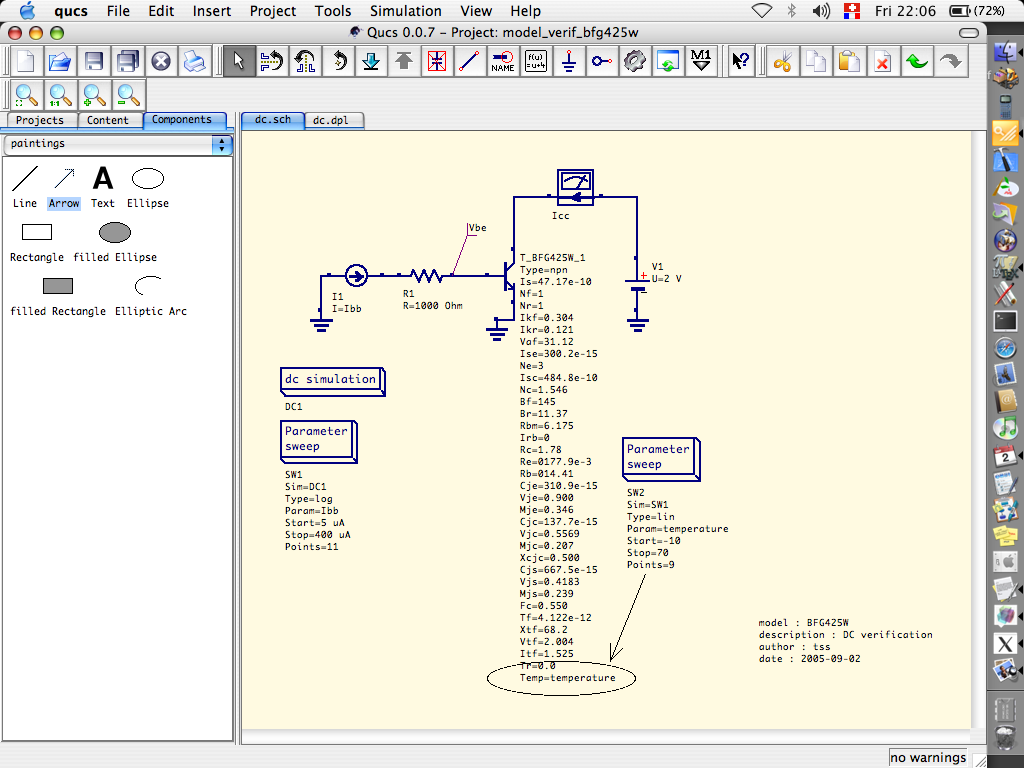
\includegraphics[scale=0.5,angle=90]{modelVerifProject}
	\caption{QUCS project for model verification}
	\label{design:pa:model:project}
\end{center}
\end{figure}

\begin{figure}[htbp]
\begin{center}
	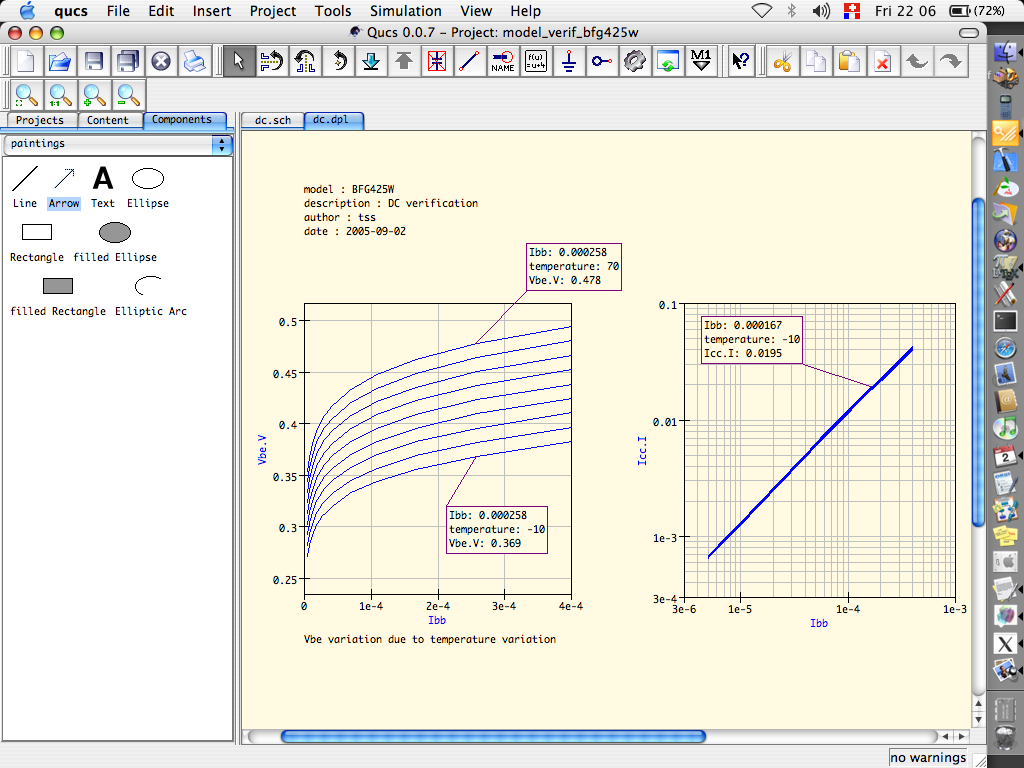
\includegraphics[scale=0.5,angle=90]{model_dc_temp}
	\caption{DC validation and temperature}
	\label{design:pa:model:dcTemp}
\end{center}
\end{figure}

For the validation we will need to use a specific bias of the device : $I_c$ should be $25 mA$, therefore $I_b$ should be $300 \mu A$

\tutsection{parasitic description of the package}

In order to simulate properly the device, you need to used the correct package, that is to say the $SOT343R$ in our case, as mentionned on the philips web site ( see fig. \ref{design:pa:model:sotDesc}).

\begin{figure}[htbp]
\begin{center}
	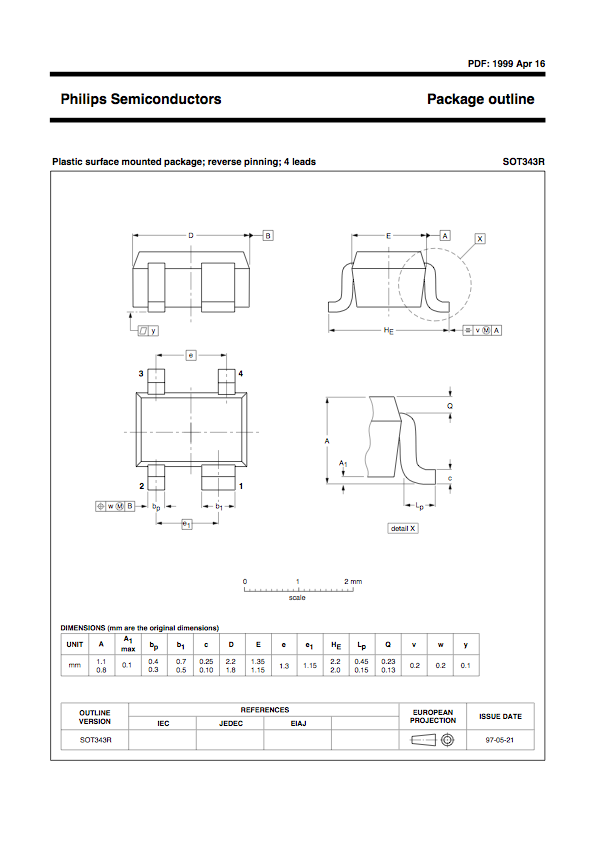
\includegraphics[scale=0.6]{sot343R}
	\caption{$SOT343R$ package description}
	\label{design:pa:model:sotDesc}
\end{center}
\end{figure}

Eventhough the device has two emitter, the model used has only one emitter. The parasitic of this model are shoyn in the spice netlist described in the choice of the transistor and reproduced in a schematic (see fig. \ref{design:pa:model:parasitSch}). These parameter are always critical to extract, either you have the knowledge to do it or then you should rely on the piece of information given by the device manucfacturer. It is also very difficult to figure out what have to be changed in such description of the device. Some fitting have been performed using 3D electromagnetic software in the time domain based on MOM methods to verify these parameters.

Philips�  fifth  generation double poly silicon wideband technology uses a steep emitter doped profile resulting in transition frequencies over 20 GHz, and with poly base contacts a low base resistance is obtained. Via the buried layer, the collector contact is brought out at the top of the die. The substrate is connected directly to the emitter package lead, resulting in improved thermal performance ( see fig \ref{design:pa:model:fifthGen}).

\begin{figure}[htbp]
\begin{center}
	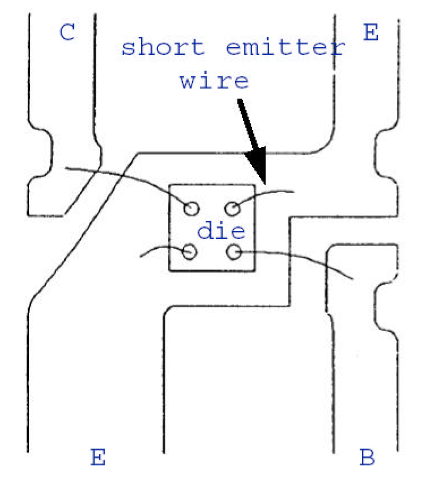
\includegraphics[scale=0.2]{fifthGen}
	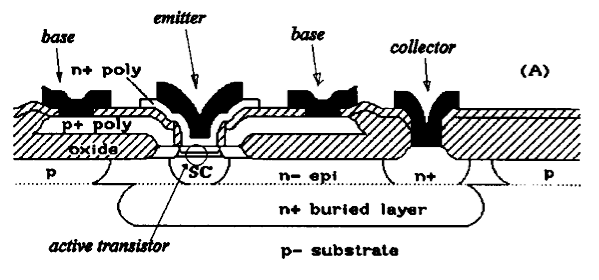
\includegraphics[scale=0.3]{silicium}
	\caption{die connection if the fifth generation transistor from philips}
	\label{design:pa:model:fifthGen}
\end{center}
\end{figure}


\begin{figure}[htbp]
\begin{center}
	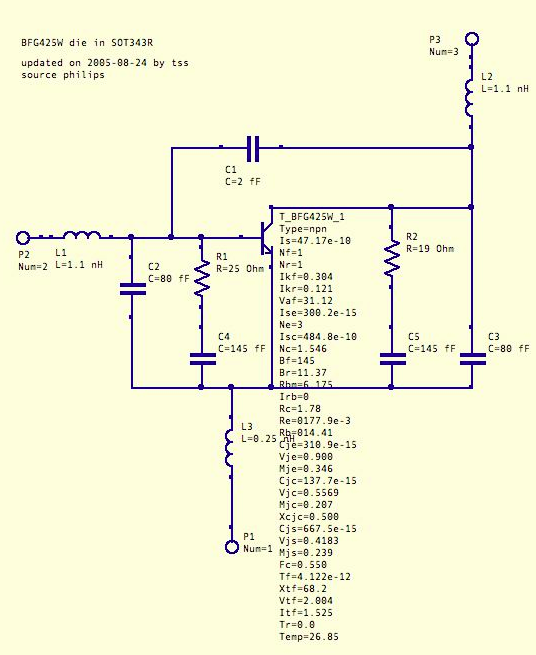
\includegraphics[scale=0.8]{bfg425Sch}
	\caption{$bfg425W$ in $sot343R$ package description}
	\label{design:pa:model:parasitSch}
\end{center}
\end{figure}

From this schematics you can edit the symbol that could be used in the next simulation file. To proceed type $F3$ or edit circuit symbol from the file menu. Simply drw a npn transistor and come back to the schematic by re-pressing $F3$.

\tutsection{small signal S parameter verification}

In this section we will need to redraw a new schematics using the model we have created, plus some extra components to place the measurements ports \footnote{We will another method when we will use the device in a real project}.

You should have a schematics like the one mentionned in fig\ref{design:pa:model:spSch}.

\begin{figure}[htbp]
\begin{center}
	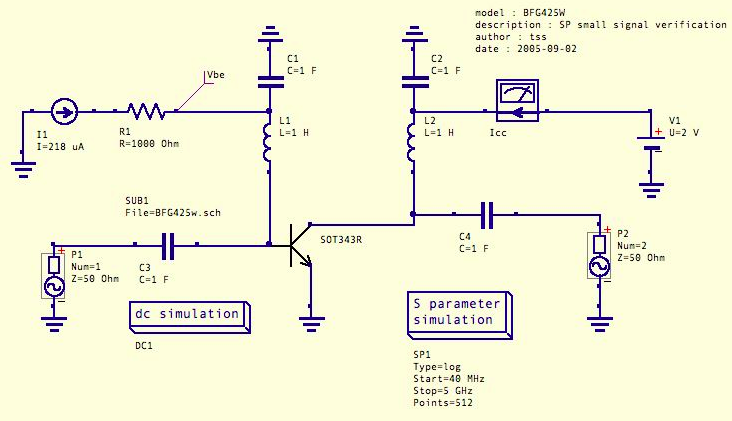
\includegraphics[scale=0.5]{model_spSch}
	\caption{schematics used for S parameters simulation}
	\label{design:pa:model:spSch}
\end{center}
\end{figure}

The components used to verify the model could be strange ( inductor of $1H$ and capacitor of $1F$ ) It is normal since we need to have a very wide band response on the circuit, and since we want to caracterize only the active device, and compare with the datasheet. An other way is to use DC bloc or DC feed or bias Tee to provide the power supply to the component. This is the right way to do it. 

you should then create a display to visualize the S parameters : generally $s_{11}$ and $s_{22}$ are in the smith and $s_{12}$ and $s_{21}$ are in polar

\begin{figure}[htbp]
\begin{center}
	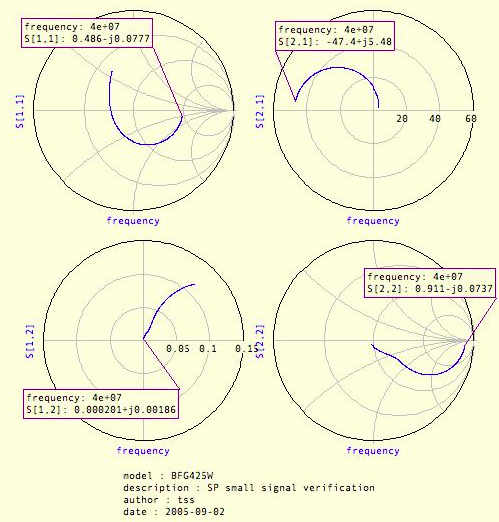
\includegraphics[scale=0.7]{model_sp}
	\caption{S parameters simulation for model verification}
	\label{design:pa:model:sp}
\end{center}
\end{figure}

We have now to compare these results with the measured parameters from philips :

\begin{verbatim}
! Filename: 225bfg425.001
! BFG425W Field C1
! V1=8.667E-001V,V2=2.000E+000V, I1=3.585E-004A, I2=2.496E-002A
!                S11              S21              S12              S22
!Freq(GHz)  Mag     Ang      Mag     Ang      Mag     Ang      Mag     Ang 
# GHz   S   MA   R 50
   0.040    0.325  -8.696   38.472 173.381    0.002  71.865    0.923  -3.072
   0.100    0.331 -23.004   37.457 164.549    0.005  83.280    0.915  -9.551
   0.200    0.315 -44.455   34.771 150.487    0.008  75.947    0.863 -18.965
   0.300    0.296 -63.008   31.364 138.811    0.012  71.608    0.794 -26.449
   0.400    0.278 -79.654   27.951 128.829    0.015  68.186    0.725 -32.076
   0.500    0.265 -94.339   24.856 120.248    0.017  65.974    0.664 -36.332
   0.600    0.254 -106.508   22.159 113.362    0.020  64.514    0.613 -39.533
   0.700    0.246 -116.820   19.885 107.530    0.022  63.362    0.569 -42.071
   0.800    0.240 -126.472   17.964 102.255    0.024  62.701    0.533 -44.121
   0.900    0.235 -134.500   16.345  97.645    0.027  61.910    0.504 -45.968
   1.000    0.232 -141.743   14.958  93.487    0.029  61.280    0.479 -47.614
   1.100    0.230 -148.265   13.770  89.661    0.031  60.570    0.457 -49.172
   1.200    0.230 -154.216   12.748  86.091    0.033  59.878    0.438 -50.696
   1.300    0.230 -159.761   11.850  82.773    0.036  59.238    0.421 -52.103
   1.400    0.231 -164.776   11.070  79.671    0.038  58.509    0.406 -53.483
   1.500    0.233 -169.782   10.383  76.687    0.040  57.719    0.392 -54.842
   1.600    0.234 -174.382    9.766  73.821    0.043  56.846    0.380 -56.285
   1.700    0.236 -178.496    9.213  71.086    0.045  56.001    0.369 -57.740
   1.800    0.238 177.334    8.725  68.404    0.047  54.999    0.358 -59.199
   1.900    0.241 173.487    8.277  65.836    0.050  53.983    0.348 -60.790
   2.000    0.244 169.856    7.874  63.295    0.052  52.923    0.338 -62.399
   2.200    0.251 162.836    7.172  58.413    0.057  50.729    0.319 -65.657
   2.400    0.259 156.208    6.578  53.682    0.062  48.414    0.301 -68.988
   2.600    0.268 150.081    6.068  49.042    0.067  45.958    0.283 -72.558
   2.800    0.277 144.221    5.628  44.575    0.072  43.380    0.266 -76.167
   3.000    0.288 138.650    5.244  40.174    0.077  40.713    0.248 -80.054
   3.500    0.319 125.843    4.470  29.452    0.090  33.634    0.204 -90.648
   4.000    0.352 113.999    3.873  18.944    0.102  26.177    0.158 -103.541
   4.500    0.389 103.406    3.406   8.713    0.113  18.415    0.113 -121.590
   5.000    0.431  92.903    3.011  -1.792    0.123   9.782    0.071 -156.899
   5.500    0.463  82.559    2.658 -11.364    0.131   2.534    0.054 148.652
   6.000    0.506  73.164    2.374 -21.684    0.138  -6.413    0.095 100.575
   6.500    0.516  66.705    2.179 -28.681    0.152 -10.089    0.112  92.309
   7.000    0.551  59.664    2.011 -37.894    0.164 -17.920    0.164  82.321
   7.500    0.610  50.773    1.808 -49.313    0.166 -29.630    0.246  65.957
   8.000    0.644  43.502    1.653 -58.585    0.172 -37.580    0.300  56.971
   8.500    0.683  35.816    1.496 -68.478    0.175 -46.984    0.361  47.167
   9.000    0.709  27.972    1.338 -77.310    0.173 -55.176    0.412  37.289
   9.500    0.736  20.858    1.212 -85.841    0.172 -63.448    0.449  29.117
  10.000    0.764  14.187    1.105 -95.600    0.173 -72.751    0.505  22.602
  10.500    0.785   7.330    0.997 -104.961    0.171 -81.774    0.554  14.956
  11.000    0.802   0.219    0.884 -113.744    0.164 -91.275    0.593   6.422
  11.500    0.815  -6.751    0.791 -122.965    0.158 -100.952    0.631  -0.521
  12.000    0.822 -13.843    0.690 -131.882    0.149 -111.108    0.667  -8.548
!     DEEMBEDDED NOISE DATA
!FREQUENCY    FMIN    GAMMA OPT        Rn
!  (GHz)      (dB)    Mag    Ang   (NORMALIZED)
\end{verbatim}


Using these parameter, we shoul compare on the sample display the modelised results and the measurements results, or directly show the error using equations. First we compare the results.

\begin{figure}[htbp]
\begin{center}
	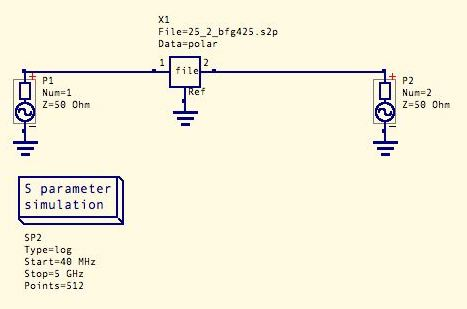
\includegraphics[scale=0.7]{model_mesureSch}
	\caption{schematics used for S parameters from manufacturer}
	\label{design:pa:model:spMeasSch}
\end{center}
\end{figure}

In the display that is used for the S parameters that we have simulated from our modelisation, you can add the results from the meaurements files by adding a measurement of $S_{i,j}$ using the right dataset with the combo box. You should obtain the difference between the two.

By doing this, you should obtain the results presented in the figure \ref{design:pa:model:mesureSp}.

\begin{figure}[htbp]
\begin{center}
	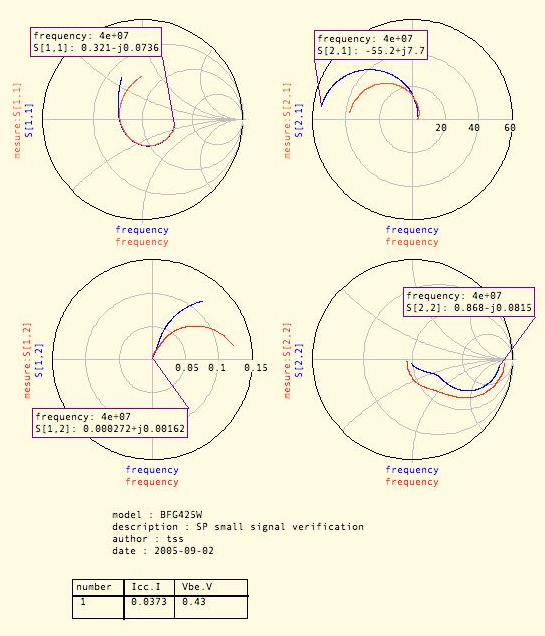
\includegraphics[scale=0.7]{model_mesureSp}
	\caption{Results from model and from meaures compared together}
	\label{design:pa:model:mesureSp}
\end{center}
\end{figure}

\bigskip

\textbf{IMPORTANT NOTE : }The differences, you should obtain are still on investigation for now.
